\documentclass[12pt,a4paper]{article}
\renewcommand{\contentsname}{Table des Matières}
\usepackage{mwe}
\usepackage[french]{babel} 
\usepackage{fancyhdr}
\usepackage{graphicx}
\usepackage{amsfonts,amssymb,amsmath} 
\usepackage{hyperref}
\usepackage[sorting=none]{biblatex}
\usepackage{subcaption}
\usepackage{soul, xcolor}
\usepackage{subfig}
\addbibresource{references.bib}
\usepackage{enumitem} 
\usepackage{geometry} 
\usepackage{float}
\geometry{hmargin=2cm,vmargin=2.5cm}
\pagestyle{fancy}
\fancyhf{} % Effacer les en-têtes et pieds de page par défaut
\fancyhead[L]{\tiny MONNOT | CHABRIT | VILPELLET | ZLOCH} % En-tête à gauche
\fancyhead[R]{\tiny Gestion quantitative 2} % En-tête à droite
\fancyfoot[C]{\thepage} % Numéro de page au centre du pied de page
\renewcommand{\headrulewidth}{0pt} % Pas de ligne sous l'en-tête
\renewcommand{\footrulewidth}{0pt} % Pas de ligne au-dessus du pied de page
\fontsize{12}{15}\selectfont % 12pt font size, 1.15 interline spacing


\begin{document}

\begin{titlepage}
	\centering
	{\LARGE \textsc{Université Paris Dauphine - PSL}\par}
	\vspace{1cm}
	{\Large\bfseries Master 272 - Ingénierie Économique et Financière \par}
    {\Large \bfseries Majeure Finance Quantitative \par}
    \vspace{1.5cm}
    {\LARGE \textsc{Discretization of continuous-time arbitrage strategies in financial markets with fractional Brownian motion}\par}
    \vspace{2cm}
	{\Large Gestion quantitative 2 : Réplication \& Extensions\par}     
    \vspace{1cm}
    \textit{Superviseurs} \\
    Mr Matthieu \textsc{GARCIN}, 
    Mr Chafic \textsc{MERHY}, 
    Mr Julien \textsc{ROYER}
	\vfill
 
	\textit{Auteurs}\par
 Matthieu \textsc{MONNOT} \\
 Paul-Antoine \textsc{CHABRIT} \\
 Jérémie \textsc{VILPELLET} \\
 Baptiste \textsc{ZLOCH}
    \vfill

    % \begin{figure}[h]
    %        \begin{subfigure}[a]{1\textwidth}
    %            \centering
    %            
\includegraphics[width=1\textwidth]{dauphine-psl_2.png}\par
    %            \end{subfigure}%
    %        \hspace{6mm}
    %\end{figure}
   % 
\includegraphics[width=0.6\textwidth]{dauphine-psl_2.png}\par
    %\includegraphics[width=0.4\textwidth]{sg.jpg}\par 
	\vfill
% Bottom of the page
	{\large  Année Académique 2023--2024\par}
\end{titlepage}


\newpage
\tableofcontents

\newpage
\section{Introduction}\label{sec:introduction}
La découverte de stratégies d'arbitrages n'est pas chose aisée, en effet, elles reposent sur de nombreuses hypothèses et ces dernières sont souvent irréalisables en pratique. Cependant l'arbitrage est un objectif pour beaucoup d'investisseurs car il permet d'engranger des profits sans risques. C'est un challenge que de nombreux hedge funds tentent de résoudre en recrutant les mathématiciens les plus performants. Il est important de distinguer l'arbitrage classique Björk (2005)\cite{bjork2005} que nous abordons ici et l'arbitrage statistiques, non traité ici. On peut de manière rigoureuse définir un arbitrage dit classique comme suit :
\begin{equation}\label{eq:arbitrage}
\begin{split}
 (i)\quad &  V_0^\Phi = 0 \\
 (ii)\quad &\mathbb{P}(V_t^\Phi \geq \text{for all}\quad t\in(0,T])=1 \\
 (iii)\quad &\mathbb{P}(V_T^\Phi>0)>0
\end{split}
\end{equation}

Cependant la théorie de valorisation des actifs contingents est majoritairement enseignée selon les hypothèses d'absence d'opportunités d'arbitrages. On peut citer notamment Black \& Scholes (1973)\cite{black1973pricing}. Ces derniers proposent d'une part un modèle de valorisation d'actifs contingents mais surtout donnent un cadre complet pour la réplication de ces mêmes actifs contingents en utilisant une stratégie bien définie basée sur un actif risqué et un actif sans risque. Leur théorie repose sur l'absence d'opportunités d'arbitrages. L'absence d'opportunités d'arbitrages est nécessaire pour l'hypothèse d'un marché complet qui stipule que dans un tel marché, tous les actifs sont réplicables. C'est d'ailleurs dans un tel marché que la probabilité risque neutre notée $\mathbb{Q}$\footnote{Loi de probabilité dans laquelle l'aversion au risque des investisseurs n'existe pas.} existe. Cette approche plutôt orientée sell-side\footnote{Le sell-side correspond à l'industrie bancaire et notamment les banques d'investissement, CIB.} qui vendent des produits dérivés possède son pendant côté buy-side\footnote{Le buy-side correspond à l'industrie de la gestion d'actifs et des hedge funds.} souvent appelé efficience de marché Fama (1970)\cite{fama1970}. L'efficience des marché considère que l'ensemble de l'information est contenu dans le prix d'un actif et par conséquent elle est accessible à tous les agents économiques. Il est donc impossible de "battre" le marché de manière durable. Cette hypothèse des marchés efficients a été vivement critiquée notamment par Malkiel (2003)\cite{malkiel2003}. Nous assistons donc de nos jours à de nombreuses remises en cause de cette complétude des marchés. 

L'émergence de nouvelles stratégies d'arbitrage et de technologies toujours plus performantes intéressent de plus en plus les investisseurs. L'utilisation d'outils souvent empreintés à la Physique fournissent également un formidable cadre pour l'élaboration de stratégies de trading. On peut également parler d'Econophysique qui mélange économie et physique, c'est un sujet de plus en plus présent en finance. 
Dans ce document nous traitons justement d'un article nommé "\textit{Discretization of continuous-time arbitrage strategies in financial markets with fractional
Brownian motion}" par Lamert et al. (2023)\cite{lamert2023discretization} qui tentent d'appliquer aux conditions réelles en incluant frictions et frais, deux stratégies d'arbitrage en temps continue. Ces stratégies sont basées sur un outil bien connu des physiciens appelé le mouvement Brownien fractionnaire (fBm) introduit par Mandelbrot \& Ness (1968)\cite{MandelbrotNess1968}. Il s'agit d'une version généralisée du mouvement Brownien standard mais dans laquel on trouve un paramètre supplémentaire, l'exposant de Hurst noté $H$ $\in [0,1]$ qui correspond à un mesure de dépendance sérielle entre les incréments. L'introduction de dépendance entre les incréments rend le processus non markovien. On définit souvent le fBm par sa covariance :
\begin{equation}\label{eq:fbm}
    \mathbb{E}[B_H(t)B_H(s)]=\frac{1}{2}(\vert t\vert^{2H}+\vert s\vert^{2H}-\vert t-s\vert^{2H})
\end{equation}
Avec $H\space [0,1]$ l'exposent de Hurst, $B_H$ le fBm dicté par le paramètre $H$, $s$ et $t$ avec $s<t$ deux indices d'incrément différents. On constate qu'en effet le propriété markovienne n'est plus vérifiée, sauf dans le cas ou $H=0.5$ ce qui est le cas d'un mouvement Brownien standard. Les stratégies d'arbitrage de cet article sont basées sur une dynamique du sous-jacent suivant un fBm pour un $H>0.5$ et donc une dépendance sérielle positive des incréments. On peut parler d'effet de momentum, Moskowitz (2011)\cite{moskowitz2011}.

La première stratégie est une stratégie introduite par Shiryaev (1998)\cite{shiryaev1998} qui consiste en l'achat et le rebalancement continu d'un actif à risque dont la dynamique est un fBm \ref{eq:fbm} et d'un actif sans risque de valeur constante 100. La seconde stratégie est une stratégie introduit par Salopek (1998)\cite{salopek1998} qui consiste en l'achat et le rebalancement continu de deux actifs à risque dont la dynamique est un fBm \ref{eq:fbm}. Cette dernière s'apparente à un long/short ou un pair trading continue entre deux actifs. Ces stratégies ont été démontrée mathématiquement comme étant un arbitrage au sens des conditions \ref{eq:arbitrage}. L'enjeu des auteurs va être ici d'étudier et de quantifier l'impact de la discrétisation, de l'introduction des coûts de frictions et de rebalancement sur le P\&L. Nous allons répliquer le papier de Lambert et al (2023)\cite{lamert2023discretization} pour confirmer les différents impacts de la discrétisation, de l'introduction des coûts de frictions et de rebalancement sur le P\&L. Nous proposeront enfin dans la section \ref{sec:extensions} des extensions ou des cas qui n'ont pas forcément été couverts par les auteurs.

\section{Réplication}\label{sec:replication}
\subsection{Mouvement Brownien fractionnaire $B_H$}\label{subsec:generationfbm}
JEREM
\subsubsection{Méthodes de génération du processus}
JEREM
\subsubsection{Demo}
Soit \( H \in [0,1] \) et \(x =  0, 1, ..., N-1  \) avec \(N \in \mathbb{N} \). On a \((\phi_i)_{i \in \mathbb{Z}} \text{ i.i.d. } \sim U([0,2\pi])\).



\subsection{Procédure de backtest}\label{subsec:backtest}
Afin de procéder à la vérification de l'arbitrage lors du passage en temps discret il est nécessaire de réaliser un backtest. En effet, les stratégies étant basées sur la génération d'un ou deux chemins de dynamiques fractionnaire, il est nécessaire d'effectuer des simulations de Monte-Carlo. Sur chacune des simulation de Monte-Carlo nous générons le ou les chemins nécessaires et nous appliquons les strategies en utilisant une boucle qui permet de garder vérifié la filtration adaptée sur nos données. Les décisions d'allocations de la stratégie étudiée sont faites à chaque itération, on calcule ensuite le changement volume, les coûts de frictions, les coûts de transactions. On obtient à la fin la valorisation historique réalisée du portefeuilles ainsi que les positions à chaque pas $t$.

\begin{figure}[H]
    \centering
    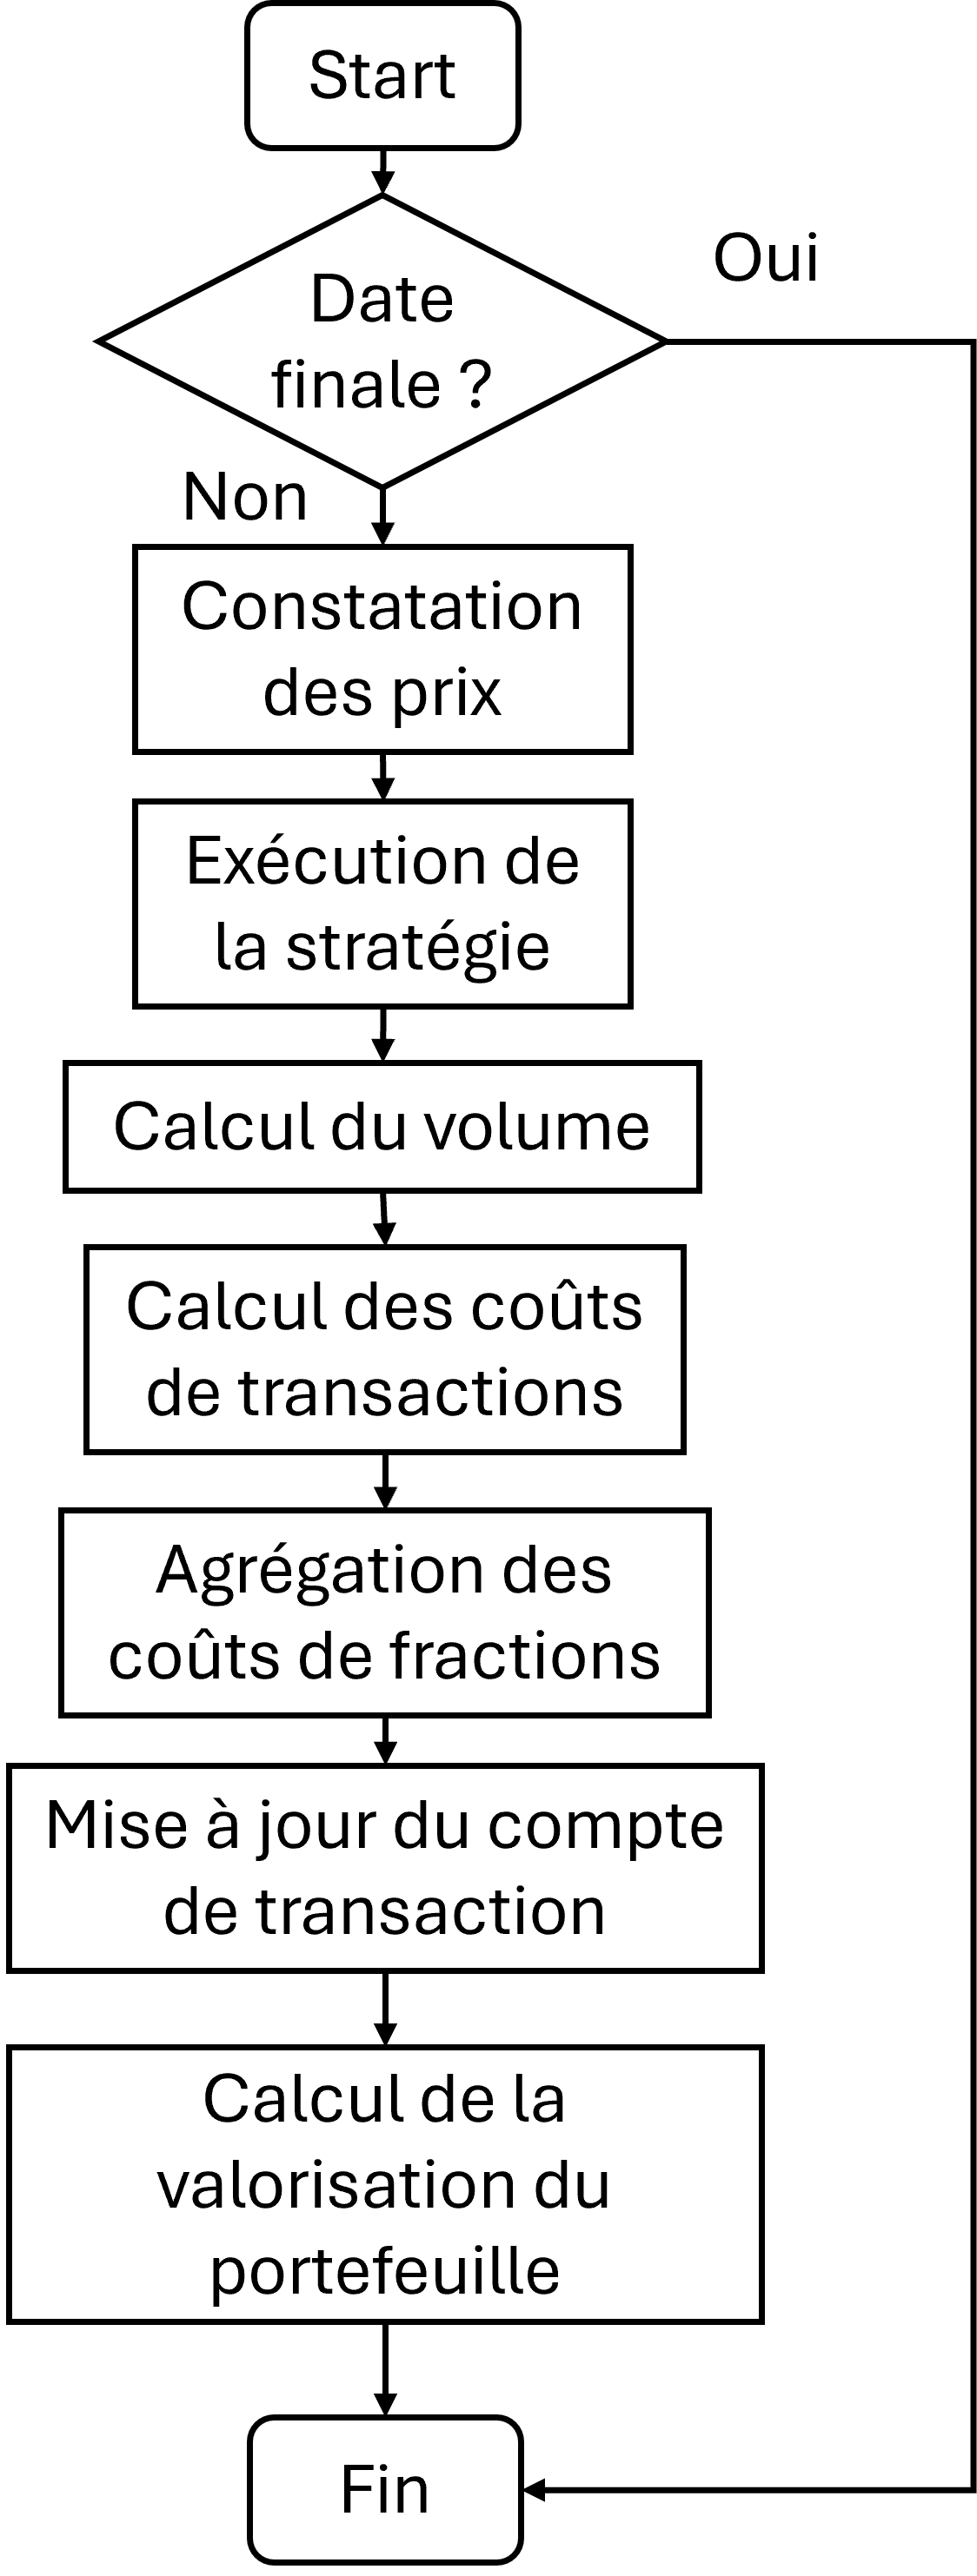
\includegraphics[width=0.25\linewidth]{img/schema_backtest.png}
    \caption{Procédure de backtest utilisée pour exécuter les stratégies}
    \label{fig:enter-label}
\end{figure}
Nous présentons ci-dessous un résume de l'ensemble des formules utilisées dans l'algorigramme ci-dessous et à fortiori dans notre procédure de calcul.


Le volume à chaque date :
\begin{equation}
     \Gamma_t^\Phi=\begin{cases}
     \sum_ {i=1}^d = \vert \Phi_1^i\vert S_0 ^i \quad \text{avec } t=t_0=0\\
     \sum_ {i=1}^d = \vert \Phi_{n+1}^i-\Phi_n^i\vert S_{t_n}^i \quad \text{avec } t=t_1,...t_{N-1} \\
     \sum_ {i=1}^d = \vert \Phi_N^i\vert S_T ^i  \quad \text{avec } t=t_N=T
     \end{cases}
\end{equation}
Les frais de transactions à chaque date :
\begin{equation}
     L_t^\Phi=l(\Gamma_t^\Phi,p)  \\
     \text { avec } \quad l(y,p)=max(p_1y,p_2)\mathbb{I}_{\{y>0\}}
\end{equation}
Avec $p=(p_1,p_2)$
\subsection{Stratégie Shiryaev}\label{subsec:strategieshiryaev}
MAN OF STEEL
\subsubsection{Résultats}\label{subsubsec:strategieshiryaevfees}
MAN OF STEEL
\subsubsection{Impact des coûts de transactions $(p_1, p_2)$}\label{subsubsec:strategieshiryaevfees}
MAN OF STEEL
\subsubsection{Impact des paramètres du modèle $(\mu, \sigma, H)$}\label{subsubsec:strategieshiryaevmodelparam}
MAN OF STEEL

\subsubsection{Impact des fréquences et de l'horizon de trading}\label{subsubsec:strategieshiryaevhorizon}
MATMAT
\subsection{Stratégie Salopek}\label{subsec:strategiesalopek}

La seconde stratégie étudiée a été introduite par Harrison et al. en 1984 puis étendue au mouvement brownien fractionnaire par Salopek en 1998. Contrairement à la précédente méthode, elle ne traite que des actifs risqués ($d\geq2$ actifs) et elle tire profit de potentielles divergences persistantes entre eux. On la décrit comme suit :

\[\Psi_{t}^{i}(\alpha,\beta) = \widehat{\Psi}_{t}^{i}(\beta) - \widehat{\Psi}_{t}^{i}(\alpha)\]
Où 
\[\widehat{\Psi}_{t}^{i}(a) = \frac{1}{d}\left(\frac{S_{t}^{i}}{M_{a}(S_{t})} \right)^{a-1} \].

$M_{a}(x)$ correspond à la moyenne de puissance d'ordre $a$ avec $x = (x_{1},\ldots,x_{d}) \in \mathbb{R}^{d}_{+}$.

\begin{align*}
    M_{a}(x) &= \left(\frac{1}{d}\sum_{i=1}^{d} (x^{i})^{a}\right)^{\frac{1}{a}} & \text{pour } a \neq 0, \\
    M_{0}(x) &= \sqrt[d]{x_{1} \cdot \ldots \cdot x_{d}} & \text{pour } a = 0.
\end{align*} \\

$M_{a}(x)$ étant une fonction croissante de $a$, pour $\alpha$ et $\beta$ tels que $\beta \geq \alpha$ on a la valeur du portefeuille de la stratégie qui s'écrit de la forme :

\[
V^{\Psi}_t = V^{\widehat{\Psi}(\beta)}_{t} - V^{\widehat{\Psi}(\alpha)}_{t} = M_{\beta}(S_{t}) - M_{\alpha}(S_{t}) \geq 0
\] \\

Salopek démontre dans son article que cette stratégie est bien un arbitrage statistique puisque qu'elle satisfait les 3 conditions : valeur de portefeuille positive en tout temps (cf. ci-dessus), apport initial nul ($V^{\Psi}_0 = M_{\beta}(s_0) - M_{\alpha}(s_0) = \Tilde{s} - \Tilde{s} = 0$) et existence d'une trajectoire à rendement strictement positif (prix des actifs presque sûrement non identiques à horizon $T$ donc $V^{\Psi}_T = M_{\beta}(S_T) - M_{\alpha}(S_T) > 0$)

\subsubsection{Résultats}\label{subsubsec:strategiesalopekresult}

Étudions à présent l'impact de la discrétisation de la stratégie sur $N$ intervalles de temps avec les paramètres par défaut et sans frais de transaction. Comparons les valeurs des portefeuilles en temps continu et temps discret tout au long de la période de trading pour quantifier les coûts de rebalancement de la stratégie. En effet, sans frais de transaction, ce sont uniquement via ces coûts de friction que les deux stratégies en temps continue et discret diffèrent. 

\begin{align}
D^{\Phi}_{t_n} = \sum_{i=0}^{d} \Phi_{n+1}^i S_{t_n}^i - \sum_{i=0}^{d} \Phi_{n}^i S_{t_n}^i &= \sum_{i=0}^{d} \left(\Phi_{n+1}^i - \Phi_{n}^i \right) S_{t_n}^i \\ 
&= \sum_{i=0}^{d} \left(\Psi_{n}^i - \Psi_{n-1}^i \right) S_{t_n}^i \quad n = 1,...,N-1
\end{align}




\subsubsection{Impact des coûts de transactions $(p_1, p_2)$}\label{subsubsec:strategiesalopekfees}
MATMAT
\subsubsection{Impact des paramètres du modèle $(\mu, \sigma, H)$}\label{subsubsec:strategiesalopekmodelparam}
BAPTBAPT
\subsubsection{Impact des fréquences et de l'horizon de trading}\label{subsubsec:strategiesalopekhorizon}
MATMAT

\subsubsection{Impact des paramètres de la stratégie $(\alpha, \beta)$}\label{subsubsec:strategiesalopekstrategyparam}
BAPTBAPT \& MATMAT

\section{Extensions}\label{sec:extensions}
\subsection{Stratégie Salopek avec $n$ assets}
\subsection{Utilisation de données réelles}
\begin{equation}
\hat{H} = -\frac{1}{2 \log(2)} \log \left( \frac{1}{2} \frac{\sum_{i=0}^{N-1} (B_H((i+1)/N) - B_H(i/N))^2}{\sum_{i=0}^{(N/2)-1} (B_H(2(i+1)/N) - B_H(2i/N))^2} \right) \label{eq:hurst_exponent}
\end{equation}

\subsection{Etude de non arbitrage pour un $H<0.5$}
PA et MATMAT ? Pair trading ? Coint \& Co ?
\section{Conclusion}\label{sec:conclusion}

\cite{lamert2023discretization}
\cite{shinozuka1972}
\cite{shiryaev1998}
\cite{yin1996}
\printbibliography

 \section{Appendix}\label{sec:appendix}
\end{document}